\chapter*{Appendix E: Eclipse Embedded CDT Preferences}
\label{E}


\addcontentsline{toc}{chapter}{Appendix E: Eclipse Embedded CDT Preferences}
\begin{figure}[H]
\begin{center}
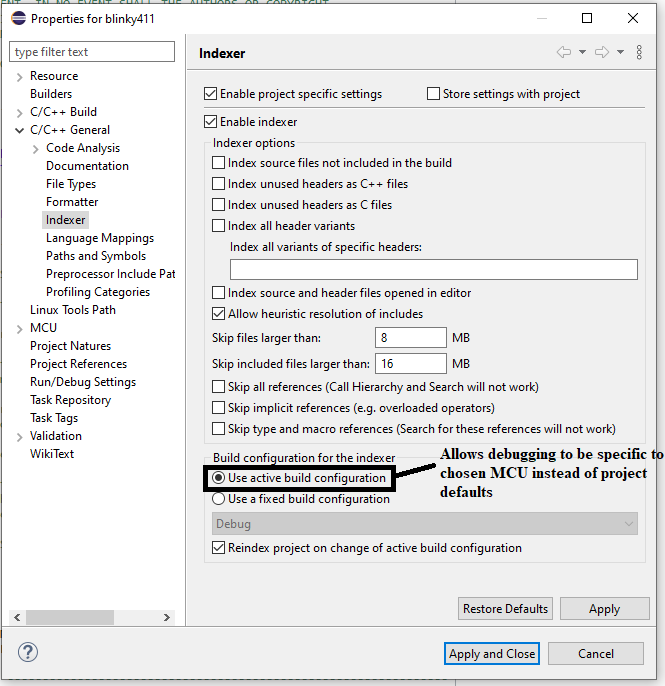
\includegraphics[width = 120mm]{p1.PNG}
\caption{Preference 1}
\label{fig:p1}
\end{center}
\end{figure}

\begin{figure}[H]
\begin{center}
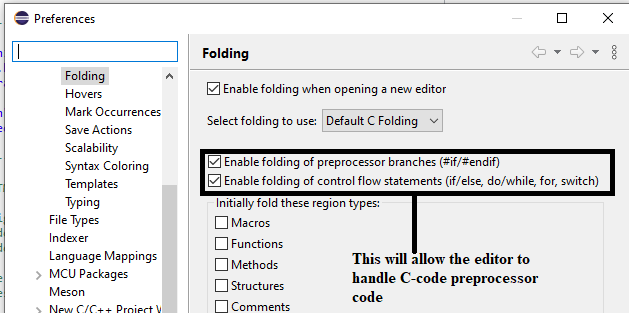
\includegraphics[width = 100mm]{p2.PNG}
\caption{Preference 2}
\label{fig:p2}
\end{center}
\end{figure}

\begin{figure}[H]
\begin{center}
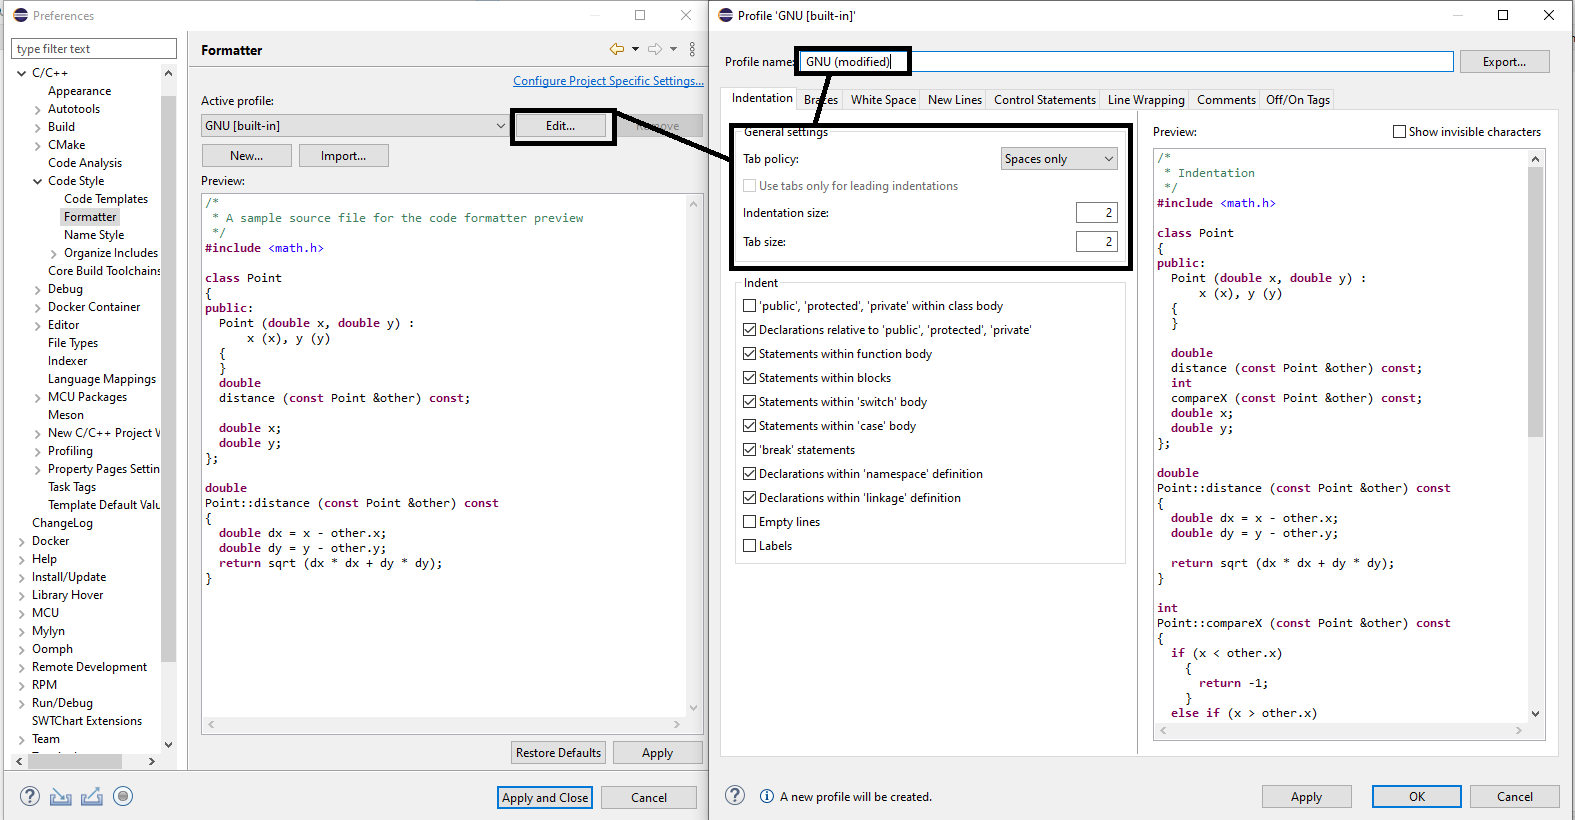
\includegraphics[scale = 0.5, angle=90]{p3.PNG}
\caption{Preference 3}
\label{fig:p3}
\end{center}
\end{figure}

\begin{figure}[H]
\begin{center}
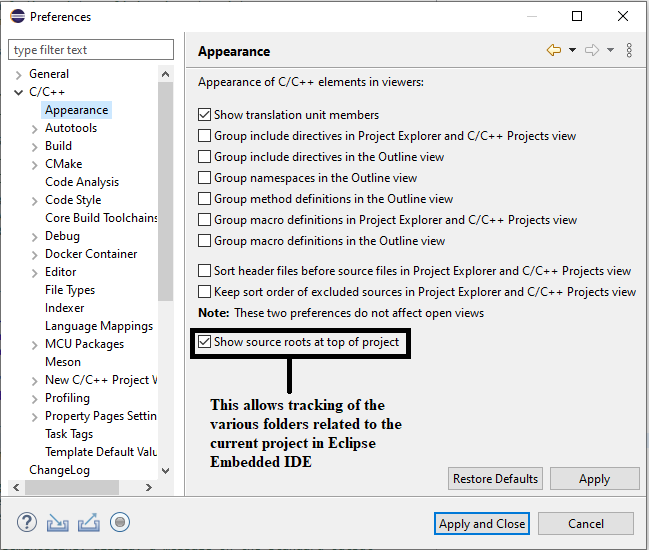
\includegraphics[width = 120mm]{p4.PNG}
\caption{Preference 4}
\label{fig:p4}
\end{center}
\end{figure}

\begin{figure}[H]
\begin{center}
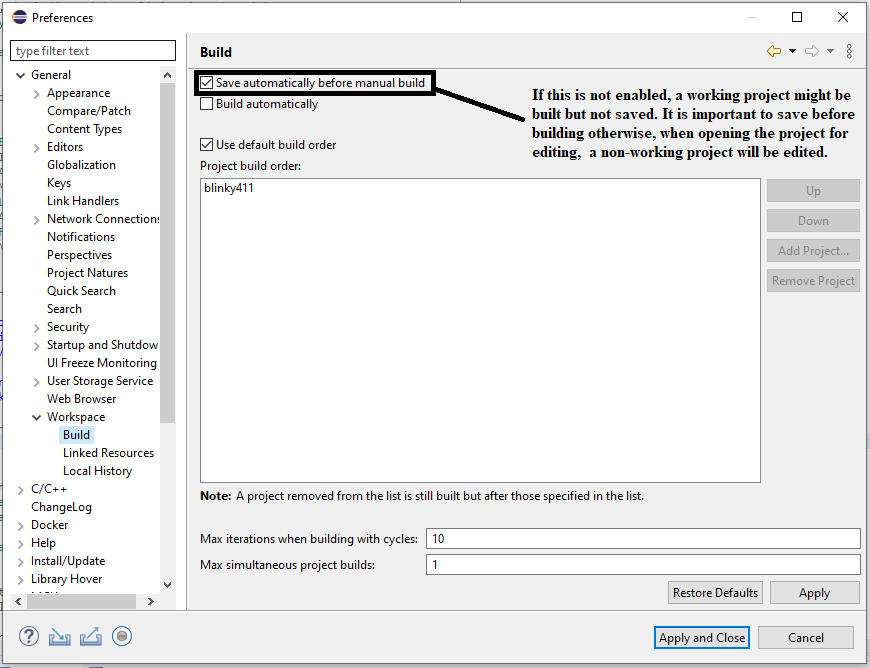
\includegraphics[width = 120mm]{p5.PNG}
\caption{Preference 5}
\label{fig:p5}
\end{center}
\end{figure}

\begin{figure}[H]
\begin{center}
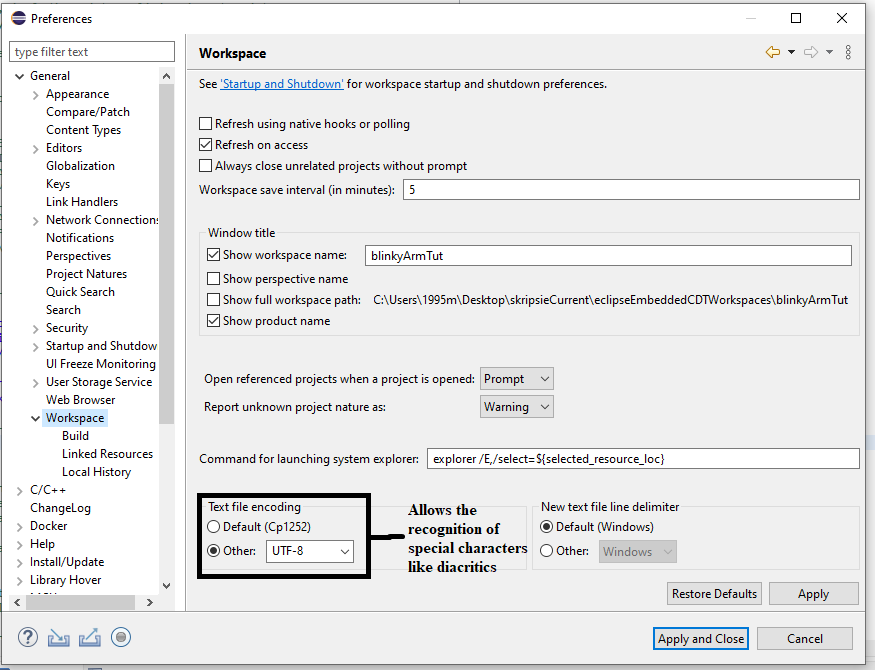
\includegraphics[width = 150mm]{p6.PNG}
\caption{Preference 6}
\label{fig:p6}
\end{center}
\end{figure}

\begin{figure}[H]
\begin{center}
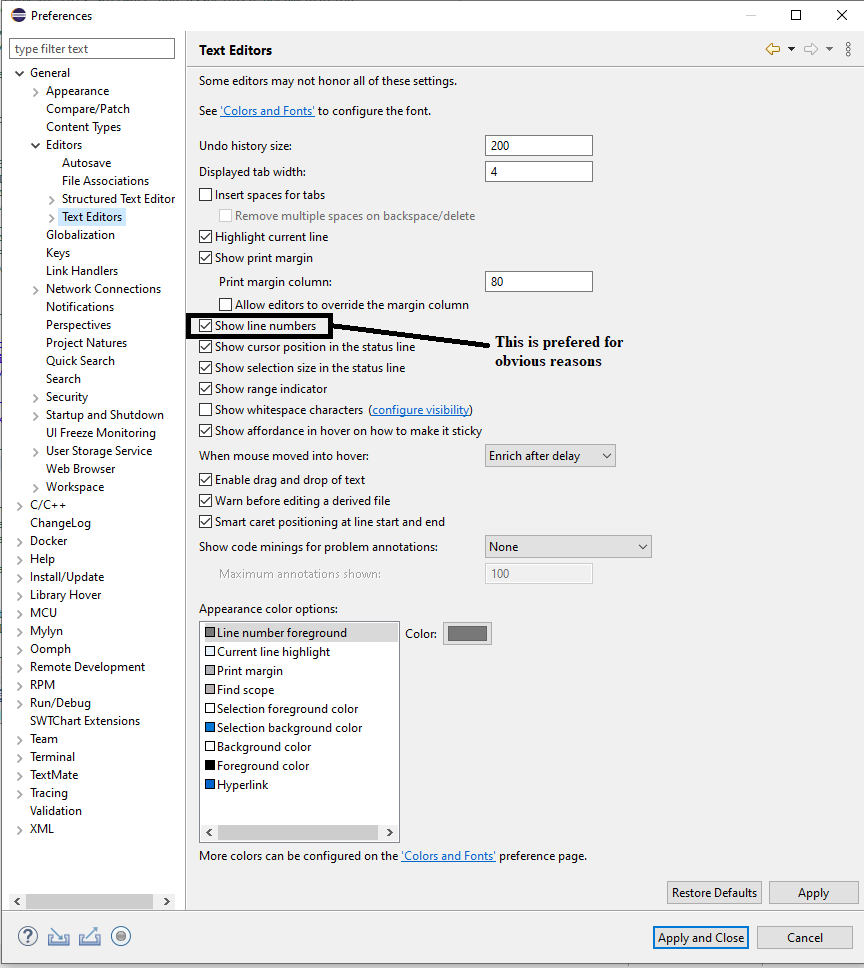
\includegraphics[width = 150mm]{p7.PNG}
\caption{Preference 7}
\label{fig:p7}
\end{center}
\end{figure}

